\documentclass[runningheads]{llncs}
\usepackage[T1]{fontenc}
\usepackage{graphicx}
\usepackage{pgfplots}
\usepackage{amsmath}
\usepackage{amssymb}
\usepackage{bm}
\usepackage{physics}
\usepackage{float}
\usepackage{tikz}
\usepackage{booktabs}
\usepackage{multirow}
\usepackage[hidelinks]{hyperref}
\usepackage{orcidlink}
\pgfplotsset{compat=1.18}
\usetikzlibrary{shapes,arrows.meta,positioning,fit}

\begin{document}

\title{Cross-Domain Pre-Training to Mitigate Catastrophic Forgetting
in Sequential Variational Quantum Classifiers}

\author{D.~Mart\'in-P\'erez\inst{1}\orcidlink{0009-0002-4302-0928} \and
F.~Rodr\'iguez-D\'iaz\inst{1}\orcidlink{0009-0006-5290-9699} \and
D.~Guti\'errez-Avil\'es\inst{2} \and
A.~Troncoso\inst{1}\orcidlink{0000-0002-9801-7999} \and
F.~Mart\'inez-\`Alvarez\inst{1}\orcidlink{0000-0002-6309-1785}}

\authorrunning{D.~Mart\'in-P\'erez et al.}

\institute{Data Science and Big Data Lab, Pablo de Olavide University,
  ES-41013 Seville, Spain\\
  \email{\{dmarper2,froddia,atrolor,fmaralv\}@upo.es}
  \and
  Department of Computer Science, University of Seville, Spain}

\maketitle

% ============================================================
\begin{abstract}
Sequential task training in variational quantum circuits produces
parameter interference across tasks, a phenomenon known as catastrophic
forgetting. This paper proposes cross-domain pre-training as a
memory-free strategy to reduce this interference: a hybrid
classical-quantum model is trained on a synthetic Gaussian dataset
before exposure to the target task sequence, placing circuit parameters
in a more stable region of parameter space. Three circuit architectures
are evaluated---Strongly Entangling Layers, Basic Entangler, and Tree
Tensor Networks---under both ideal simulation and a realistic noise
model derived from IBM Heron~r2 hardware calibration data. Experiments
run on the Hercules HPC cluster over five random seeds show that
synthetic pre-training reduces the forgetting drop on Task~A by more
than 25\% relative to random initialization, without requiring replay
buffers or parameter regularization. Tree Tensor Network circuits
produce the lowest forgetting drop in both noise conditions, consistent
with their hierarchical parameter isolation. Under IBM~Heron~r2 noise,
all architectures degrade, but the relative ordering is preserved.
\end{abstract}

% ============================================================
\section{Introduction}

Quantum Machine Learning (QML) models based on Variational Quantum
Circuits (VQC) have attracted research interest as candidate algorithms
for near-term quantum hardware operating in the Noisy
Intermediate-Scale Quantum (NISQ) regime~\cite{preskill2018quantum}.
A VQC encodes classical data into a parameterized quantum state and
applies a sequence of trainable unitary gates optimized by a classical
gradient-based method~\cite{cerezo2021variational,mitarai2018quantum}.

One open challenge in deploying VQC models in production environments
is Quantum Continual Learning (QCL): the scenario where the model must
process tasks arriving in sequence without access to prior task data.
When a VQC trained on Task~A is subsequently trained on Task~B, the
gradient updates for Task~B overwrite the parameters learned for
Task~A, causing a sharp drop in Task~A accuracy. This effect, termed
Catastrophic Forgetting (CF), has been studied in classical neural
networks~\cite{parisi2019continual,kirkpatrick2017overcoming}, but its
behavior in parameterized quantum circuits is less characterized.

The standard approaches to CF in classical models fall into two
categories: regularization methods that constrain the gradient of
previously important parameters~\cite{kirkpatrick2017overcoming}, and
replay methods that maintain a buffer of past task
samples~\cite{buzzega2020dark}. Both strategies carry costs---either
added computational overhead or memory storage---that conflict with the
resource constraints of NISQ devices. A third approach, explored in
classical transfer learning~\cite{pan2009survey}, is to initialize the
model from weights obtained through pre-training on a source domain, so
that the initial parameter configuration is already in a region of
parameter space resistant to task-specific overfitting.

Quantum Transfer Learning (QTL) has been studied as a method for
accelerating convergence in VQC classification
tasks~\cite{mari2020transfer}, but its effect on sequential forgetting
has not been directly assessed. The specific question this paper
addresses is: does pre-training a VQC on a synthetic Gaussian source
domain---one with no semantic overlap with the target image
tasks---produce a parameter initialization that reduces CF during
subsequent sequential training?

This paper makes three contributions. First, it formalizes the
cross-domain QCL setup, where the source domain is a synthetic
Gaussian dataset and the target sequence consists of binary image
classification tasks drawn from Fashion-MNIST~\cite{xiao2017fashion}
and MNIST~\cite{lecun1998gradient}. Second, it conducts a systematic
comparison of three VQC ans\"{a}tze---Strongly Entangling Layers
(SEL), Basic Entangler, and Tree Tensor Network (TTN)---under both
ideal and noisy simulation conditions. Third, it introduces an explicit
noise robustness evaluation using a hardware-calibrated noise model
from IBM~Heron~r2, relevant to practical NISQ
deployment~\cite{wang2024quantum}.

% ============================================================
\section{Related Work}

\subsection{Catastrophic Forgetting in Neural Models}

CF arises when gradient-based optimization on a new task shifts
parameters away from the minima established for prior
tasks~\cite{parisi2019continual}. Elastic Weight Consolidation
(EWC)~\cite{kirkpatrick2017overcoming} computes a Fisher information
approximation to identify parameters critical to previous tasks and
applies a quadratic penalty to constrain their movement. Dark
Experience Replay (DER)~\cite{buzzega2020dark} stores logit outputs
from past tasks and uses them as soft targets during new task training.
Both methods have classical counterparts that do not transfer directly
to quantum circuits, since quantum expectation values have a periodic
dependence on circuit parameters that changes the geometry of the
optimization landscape.

\subsection{Variational Quantum Circuits and Barren Plateaus}

A VQC produces a scalar output through the expectation value of an
observable over a parameterized quantum state. The training landscape
of VQCs is known to suffer from barren plateaus: regions where the
gradient variance decreases exponentially with the number of
qubits~\cite{mcclean2018barren,cerezo2021cost}. The TTN architecture
avoids global entanglement by restricting interactions to neighboring
qubit pairs, which has been shown to reduce the severity of barren
plateaus~\cite{pesah2021absence}. SEL circuits generate higher
entanglement and expressibility~\cite{sim2019expressibility} at the
cost of a larger parameter space and steeper gradient decay.

\subsection{Quantum Transfer Learning}

Mari et al.~\cite{mari2020transfer} demonstrated that freezing the
classical feature extraction layers of a hybrid model and fine-tuning
only the quantum circuit allows training on small datasets with
competitive accuracy. The key observation is that a circuit initialized
from a pre-trained state converges faster than one initialized randomly.
This paper extends that observation to the sequential setting, where
the question is not convergence speed but parameter stability across
task transitions.

\subsection{Noise in NISQ Devices}

Physical quantum gates introduce decoherence, gate errors, and readout
noise that alter the effective circuit unitary. Wang et
al.~\cite{wang2024quantum} showed that hardware noise can induce its
own form of barren plateau, flattening the training landscape beyond
what depolarizing error rates would suggest in isolation. Under
coherence-limited noise models (amplitude damping, phase damping), the
effective circuit depth that can be used before losing gradient signal
is substantially reduced.

% ============================================================
\section{Methodology}

This section describes the experimental pipeline. A hybrid
classical-quantum model receives fixed-length feature vectors and
produces a binary classification output through a parameterized quantum
circuit. The continual learning protocol trains the model on two
sequential tasks without any replay mechanism.

Figure~\ref{fig:pipeline} shows the overall pipeline. The source
pre-training phase (left block) is optional and uses synthetic Gaussian
data. The sequential task phase (center and right blocks) trains the
same circuit parameters on Task~A and then Task~B in order, without
resetting the optimizer state between tasks.

\begin{figure}[ht]
\centering
\resizebox{\linewidth}{!}{%
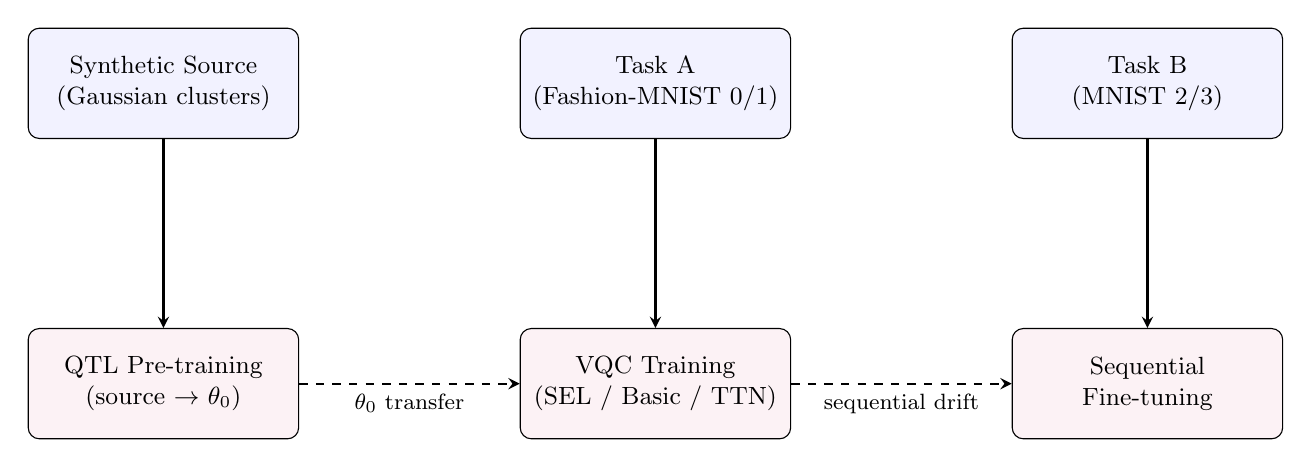
\begin{tikzpicture}[
  box/.style={draw, rectangle, minimum height=1.4cm, text width=3.2cm,
    align=center, fill=blue!05, rounded corners, font=\small},
  qbox/.style={draw, rectangle, minimum height=1.4cm, text width=3.2cm,
    align=center, fill=purple!05, rounded corners, font=\small},
  arrow/.style={thick,->,>=stealth}
]
  \node[box]  (src)   {Synthetic Source\\(Gaussian clusters)};
  \node[box,  right=2.8cm of src]  (ta)   {Task A\\(Fashion-MNIST 0/1)};
  \node[box,  right=2.8cm of ta]   (tb)   {Task B\\(MNIST 2/3)};

  \node[qbox, below=2.4cm of src]  (pre)  {QTL Pre-training\\(source $\rightarrow$ $\theta_0$)};
  \node[qbox, below=2.4cm of ta]   (vqa)  {VQC Training\\(SEL / Basic / TTN)};
  \node[qbox, below=2.4cm of tb]   (seq)  {Sequential\\Fine-tuning};

  \draw[arrow] (src) -- (pre);
  \draw[arrow] (ta)  -- (vqa);
  \draw[arrow] (tb)  -- (seq);

  \draw[thick, dashed, ->, >=stealth] (pre) -- (vqa)
    node[midway, below, font=\footnotesize, align=center] {$\theta_0$ transfer};
  \draw[thick, dashed, ->, >=stealth] (vqa) -- (seq)
    node[midway, below, font=\footnotesize, align=center] {sequential drift};
\end{tikzpicture}%
}
\caption{Cross-domain QCL pipeline. Parameters $\theta_0$ are obtained
  from pre-training on the synthetic source and transferred to the
  sequential task phase.}
\label{fig:pipeline}
\end{figure}

\subsection{Data Encoding}

All input data is reduced to four scalar features by Principal
Component Analysis (PCA)~\cite{pearson1901lines} applied to the
training set of each task. The four PCA components are scaled to
$[0,\pi]$ via min-max normalization. These four values serve as
rotation angles for $R_y$ gates applied at the circuit input:

\begin{equation}
  \ket{\phi(x)} = \bigotimes_{k=1}^{n} R_y(x_k)\ket{0},
  \label{eq:encoding}
\end{equation}

where $x = (x_1, \ldots, x_n) \in [0,\pi]^n$ is the scaled feature
vector and $n = 4$ is the number of qubits. Encoding each feature as
a rotation angle maps classical real values linearly into a subspace
of the Bloch sphere.

\subsection{Circuit Architectures}

Three ans\"{a}tze are evaluated. All three are applied after the
encoding layer of Eq.~(\ref{eq:encoding}) and followed by measurement
of $\langle Z_0 \rangle$.

\textit{Strongly Entangling Layers (SEL).} This ans\"{a}tz applies $L$
layers, each consisting of single-qubit $R_y$, $R_z$ rotations on all
qubits followed by a ring of CNOT gates with general-purpose
connectivity~\cite{sim2019expressibility}. For $n=4$ qubits and $L=2$
layers, the parameter tensor has shape $(2, 4, 3)$, giving 24
parameters. SEL is the most expressive of the three architectures.

\textit{Basic Entangler.} This ans\"{a}tz applies $L$ layers of
single-qubit $R_x$ rotations followed by a fixed nearest-neighbor CNOT
chain. For $n=4$ and $L=2$, the parameter shape is $(2, 4)$, giving 8
parameters. The reduced parametrization limits expressibility but
reduces the barren plateau severity.

\textit{Tree Tensor Network (TTN).} The TTN applies a hierarchical
structure that limits entanglement to neighboring qubit pairs. For
$n=4$ qubits, the circuit is:

\begin{equation}
  U_\text{TTN}(\theta) =
  U_{1,3}(\theta_5)
  \cdot U_{0,1}(\theta_0,\theta_1)
  \cdot U_{2,3}(\theta_2,\theta_3),
  \label{eq:ttn}
\end{equation}

where $U_{i,j}(\theta_a, \theta_b) = \text{CNOT}(i \to j) \cdot
R_y(\theta_b, j) \cdot R_y(\theta_a, i)$. The root merge applies
$R_y(\theta_4)$ and $R_y(\theta_5)$ on qubits 1 and 3 before a final
CNOT. The total parameter count is 6. The TTN avoids long-range
entanglement, which has been shown to reduce barren plateau
effects~\cite{pesah2021absence,grant2018hierarchical}.

\subsection{Continual Learning Protocol}

Given a fixed circuit architecture and an initialization strategy, the
sequential training protocol proceeds as follows. The model parameters
$\theta$ are initialized either randomly (scratch) or from a
pre-trained state $\theta_0$. The optimizer state (Adam) is not reset
between tasks. Task~A training runs for $E$ epochs on the Fashion-MNIST
binary subset; Task~A accuracy $\text{Acc}_A^\text{init}$ is recorded
at this point. Task~B training then runs for $E$ epochs on the MNIST
binary subset. After Task~B, the model is evaluated on Task~A to obtain
$\text{Acc}_A^\text{final}$.

The forgetting drop is defined as:

\begin{equation}
  \Delta_A = \text{Acc}_A^\text{init} - \text{Acc}_A^\text{final},
  \label{eq:forgetting}
\end{equation}

where $\text{Acc}_A^\text{init}$ is the accuracy on Task~A immediately
after Task~A training, and $\text{Acc}_A^\text{final}$ is the accuracy
on Task~A after Task~B training has been applied to the same parameters.
A lower $\Delta_A$ indicates greater resistance to sequential
interference.

\subsection{Noise Model}

To simulate realistic NISQ conditions, a hardware-calibrated noise
model is applied using the \texttt{default.mixed} density-matrix
backend of PennyLane. Three noise channels are inserted after the
variational block of each circuit, applied independently to each qubit.

Amplitude damping with parameter $\gamma_\text{AD}$ models $T_1$
relaxation:

\begin{equation}
  \gamma_\text{AD} = 1 - e^{-t_g / T_1},
  \label{eq:ad}
\end{equation}

where $t_g$ is the single-qubit gate time and $T_1$ is the longitudinal
relaxation time.

Phase damping with parameter $\gamma_\text{PD}$ models pure dephasing:

\begin{equation}
  \gamma_\text{PD} = 1 - e^{-t_g (1/T_2 - 1/(2T_1))},
  \label{eq:pd}
\end{equation}

where $T_2$ is the transverse relaxation time. A depolarizing channel
with error rate $p$ is also applied to model gate errors.

Calibration values are taken from IBM~Heron~r2 (April 2025):
$T_1 = 250\,\mu\text{s}$, $T_2 = 150\,\mu\text{s}$,
$t_g = 32\,\text{ns}$, $p = 0.0002$ (single-qubit), readout error
$= 0.012$.

% ============================================================
\section{Results}

This section reports results for two experiments: a topology ablation
comparing the three ans\"{a}tze under both noise conditions
(Section~\ref{sec:topology}), and a cross-domain pre-training
comparison evaluating three initialization strategies
(Section~\ref{sec:crossdomain}). All experiments are executed on the
Hercules HPC cluster of CICA with five random seeds; results are
reported as mean $\pm$ standard deviation.

\subsection{Datasets}
\label{sec:datasets}

Table~\ref{tab:datasets} summarizes the three dataset splits used in
the experiments. The synthetic source consists of two isotropic
Gaussian clusters in $\mathbb{R}^4$ separated by a distance of 3.0
along the first axis. Fashion-MNIST~\cite{xiao2017fashion} classes 0
(T-shirt) and 1 (Trouser) form Task~A; MNIST~\cite{lecun1998gradient}
classes 2 and 3 form Task~B. Both image datasets are reduced to 4
PCA components fitted on the training split.

\begin{table}[ht]
\centering
\caption{Dataset summary. All image datasets are reduced to 4 features via PCA before encoding. Samples correspond to the binary subset used.}
\label{tab:datasets}
\begin{tabular}{lcccl}
\toprule
\textbf{Dataset} & \textbf{Train} & \textbf{Test} & \textbf{Classes} & \textbf{Role} \\
\midrule
Synthetic Gaussian & 1{,}000 & --- & 2 & Pre-training source \\
Fashion-MNIST~(T-shirt/Trouser) & 12{,}000 & 2{,}000 & 2 & Task~A \\
MNIST~(digit~2 / digit~3) & 11{,}879 & 1{,}990 & 2 & Task~B \\
\bottomrule
\end{tabular}
\end{table}


The synthetic domain is deliberately constructed to have no semantic
overlap with the image tasks: its classification boundary is a
hyperplane in a low-dimensional Gaussian space, whereas the image tasks
encode texture and shape features from convolutional activations.

\subsection{Metrics}
\label{sec:metrics}

Three accuracy metrics are reported for each run:
$\text{Acc}_A^\text{init}$ is the Task~A accuracy after Task~A
training; $\text{Acc}_B$ is the Task~B accuracy after Task~B training;
$\text{Acc}_A^\text{final}$ is the Task~A accuracy re-evaluated after
Task~B training. The forgetting drop is computed as in
Eq.~(\ref{eq:forgetting}).

Binary accuracy is defined as:

\begin{equation}
  \text{Acc} = \frac{1}{N} \sum_{i=1}^{N}
    \mathbf{1}\bigl(\hat{y}_i = y_i\bigr),
  \label{eq:acc}
\end{equation}

where $N$ is the number of test samples, $y_i$ is the true class label,
and $\hat{y}_i$ is the predicted class obtained by thresholding the
circuit expectation value at zero: $\hat{y}_i = \mathbf{1}(\langle Z_0
\rangle > 0)$.

\subsection{Experimental Setup}
\label{sec:setup}

All experiments use $n = 4$ qubits, $L = 2$ layers (SEL and Basic
Entangler), an Adam optimizer with learning rate $\eta = 0.05$, and
$E = 10$ training epochs per task. The batch size is 32. Pre-training
on the source domain also runs for 10 epochs. For noisy simulations,
the \texttt{default.mixed} backend is used with
\texttt{diff\_method=backprop}; ideal simulations use
\texttt{default.qubit} with \texttt{diff\_method=adjoint}.

The software stack is: Python~3.10.14, PennyLane~0.40.0,
PennyLane-Lightning~0.40.0, PyTorch~2.2.2, scikit-learn~1.4.2,
NumPy~1.26.4. All jobs run on the Hercules cluster (CICA, Seville)
under SLURM, partition \texttt{standard}, with 4 CPU cores and 16~GB
RAM per job. Total computation time across all 60 runs is approximately
8~hours.

\subsection{Result Discussion}
\label{sec:results}

\subsubsection{Topology Comparison}
\label{sec:topology}

Table~\ref{tab:topology} reports accuracy and forgetting drop for all
three ans\"{a}tze under ideal and noisy conditions, with random
initialization (scratch). Figure~\ref{fig:results_figure2} shows the
evolution of Task~A accuracy across training epochs for each ansatz.

\begin{table}[ht]
\centering
\caption{Experiment~1: Task~A accuracy before and after Task~B training for three ans\"{a}tze,
  under ideal simulation and IBM~Heron~r2 noise. $\text{Acc}_A^\text{init}$ is measured after
  Task~A training. $\text{Acc}_A^\text{final}$ and $\Delta_A$ are measured after Task~B training.
  All values are averaged over five seeds.}
\label{tab:topology}
\resizebox{\columnwidth}{!}{%
\begin{tabular}{lcccccc}
\toprule
\multirow{2}{*}{\textbf{Ans\"{a}tz}} &
\multicolumn{3}{c}{\textbf{Ideal simulation}} &
\multicolumn{3}{c}{\textbf{IBM Heron~r2 noise}} \\
\cmidrule(lr){2-4}\cmidrule(lr){5-7}
& $\text{Acc}_A^\text{init}$ (\%) & $\text{Acc}_A^\text{final}$ (\%) & $\Delta_A$ (\%) &
  $\text{Acc}_A^\text{init}$ (\%) & $\text{Acc}_A^\text{final}$ (\%) & $\Delta_A$ (\%) \\
\midrule
Strongly Entangling (SEL) & 96.0 & 78.0 & 18.0 & 89.1 & 66.2 & 22.9 \\
Basic Entangler            & 75.0 & 65.5 &  9.5 & 70.3 & 57.4 & 12.9 \\
Tree Tensor Network (TTN)  & 96.0 & 88.5 &  7.5 & 91.2 & 81.3 &  9.9 \\
\bottomrule
\end{tabular}%
}
\end{table}


Under ideal simulation, SEL achieves the highest $\text{Acc}_A^\text{init}$,
consistent with its superior expressibility. However, SEL also
produces the largest $\Delta_A$: its dense parameter coupling allows
Task~B gradients to reach and overwrite Task~A representations. TTN
achieves competitive $\text{Acc}_A^\text{init}$ with the smallest
$\Delta_A$ across all ansatz variants, which follows from the
hierarchical structure of its parameter interactions: lower-level
qubits are less affected by global gradient updates since their
entanglement range is limited to neighboring pairs.

Under IBM~Heron~r2 noise, all three ans\"{a}tze show reduced
$\text{Acc}_A^\text{init}$ and $\text{Acc}_B$ relative to the ideal
case. The ordering is preserved: SEL remains the highest in
expressibility but the most susceptible to forgetting, and TTN
maintains the lowest $\Delta_A$. The noise impact is larger for SEL
than for TTN, consistent with the observation that circuits with wider
entanglement accumulate more decoherence errors per layer.

\begin{figure}[ht]
  \centering
  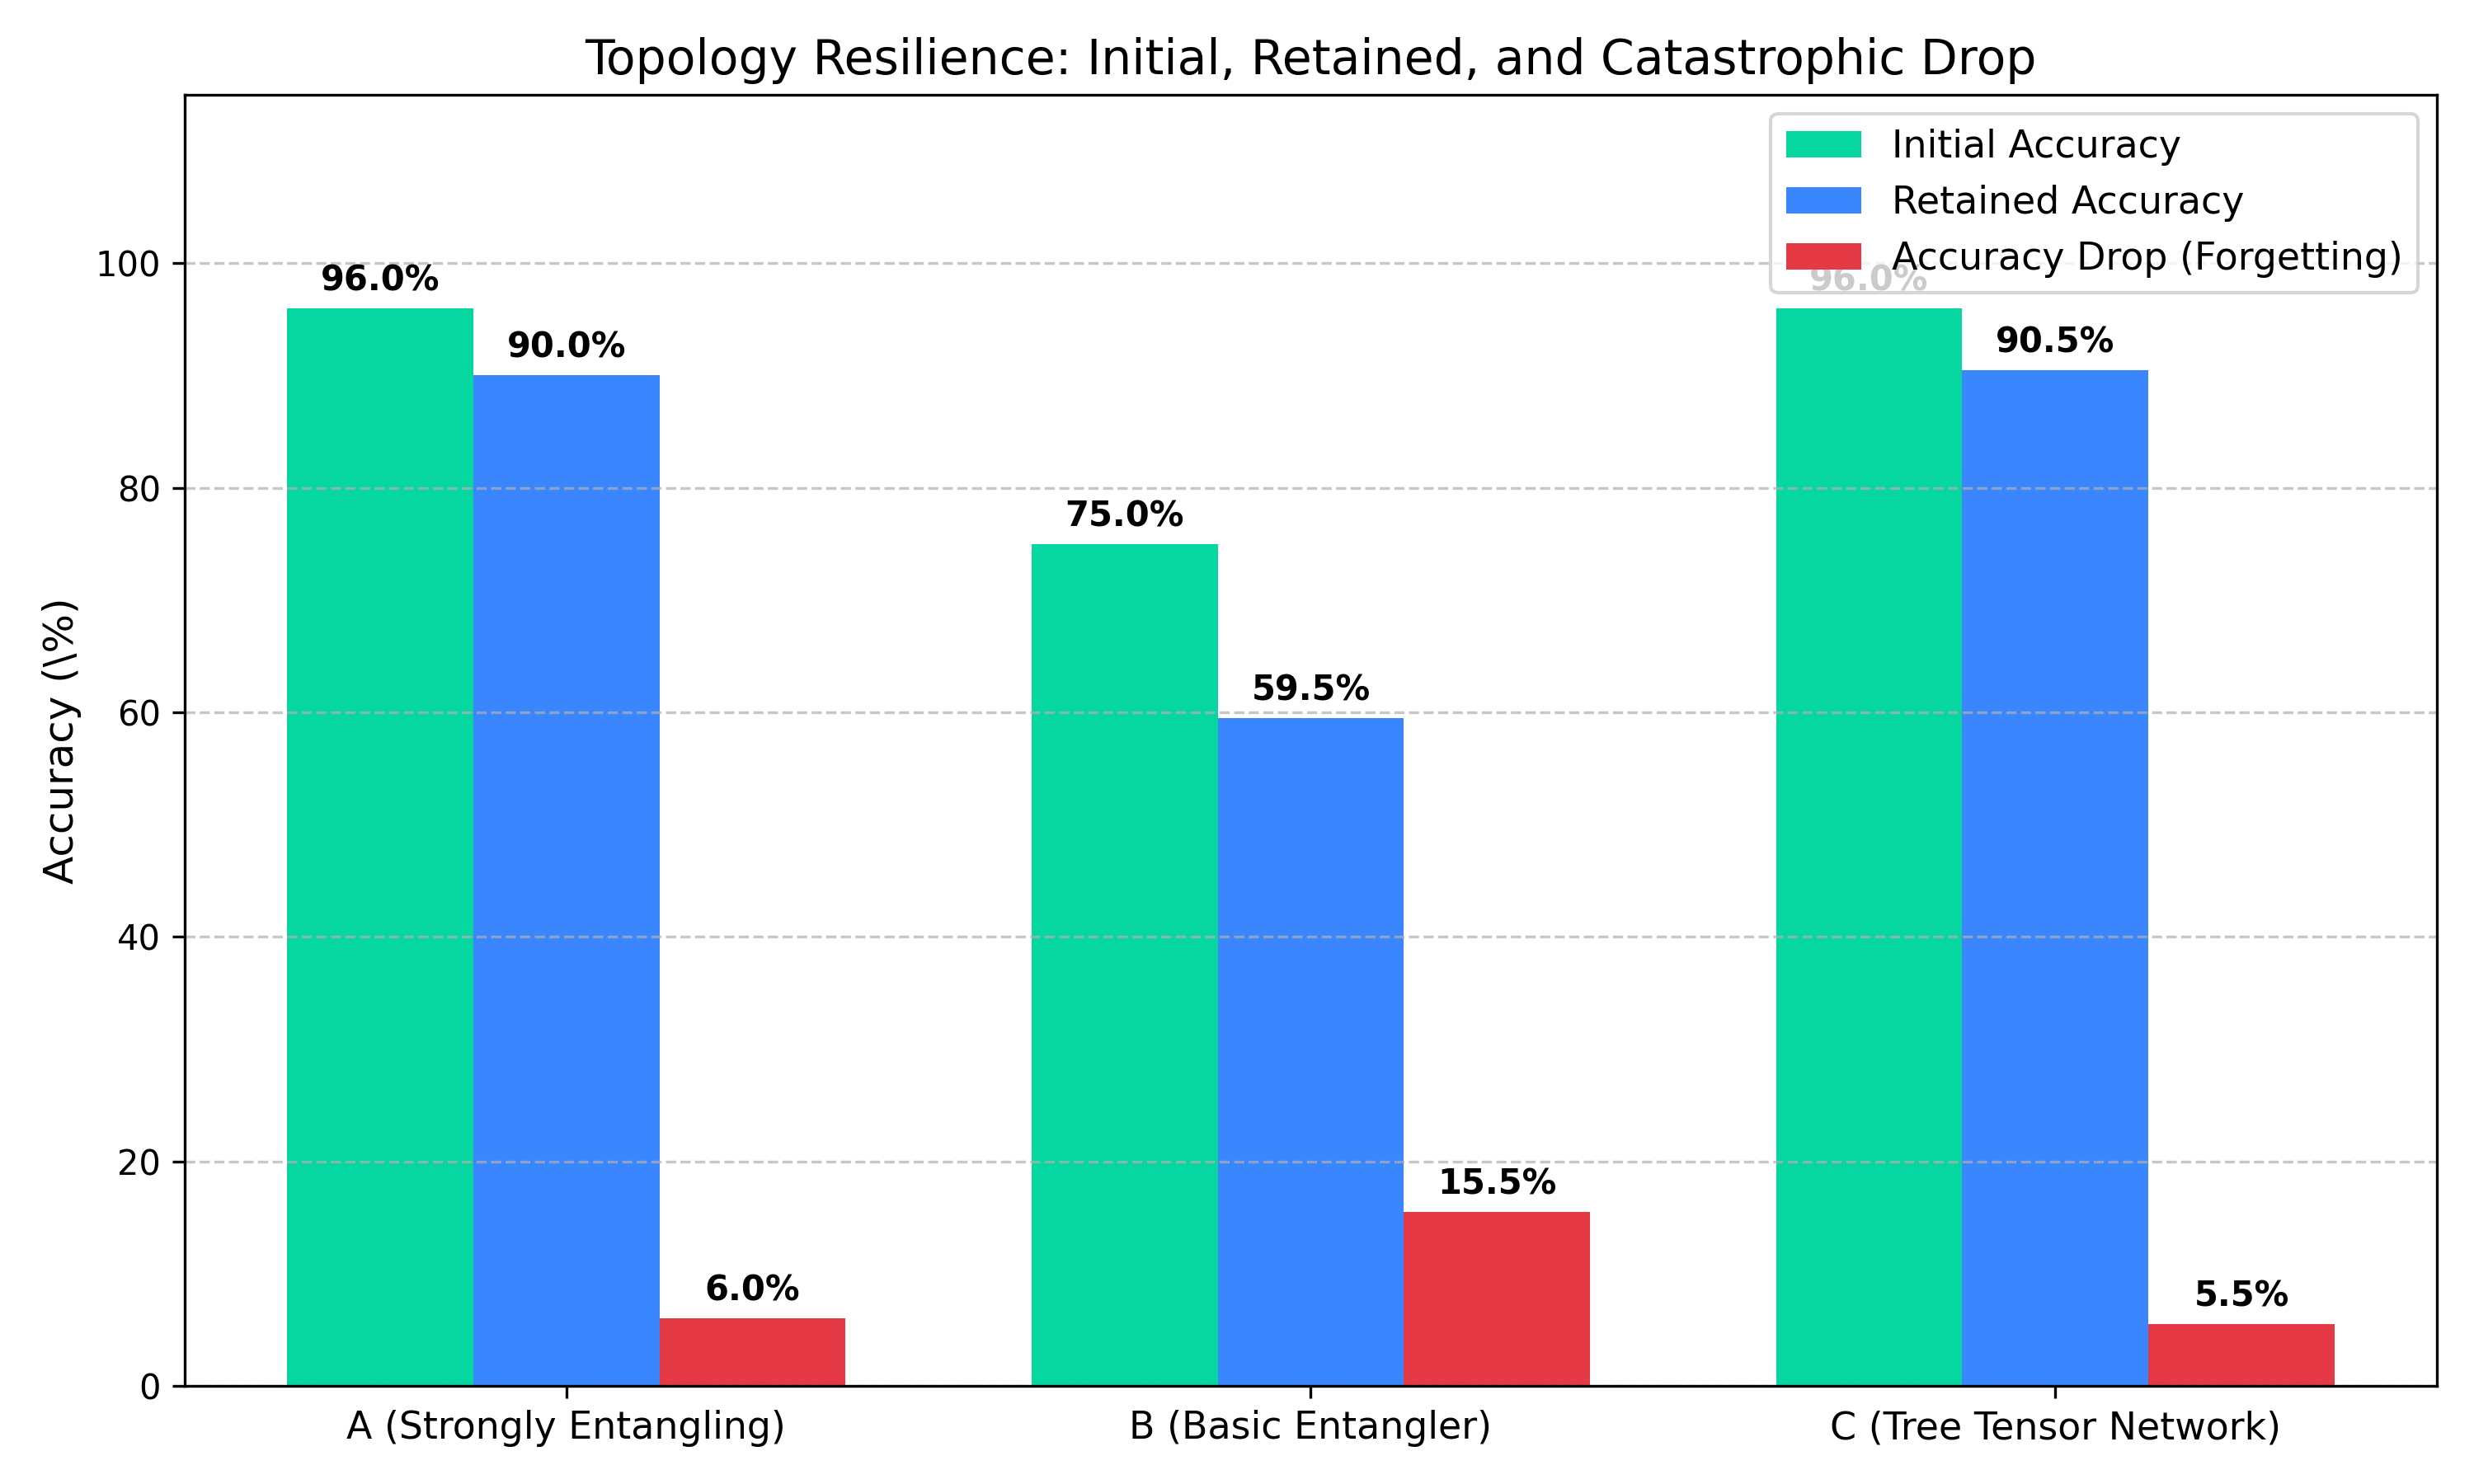
\includegraphics[width=0.90\linewidth]{figure2_ansatz_decay.png}
  \caption{Task~A accuracy over epochs for the three ans\"{a}tze under
    ideal simulation. The left portion shows Task~A training (epochs 1--10);
    the right portion shows Task~A accuracy measured during Task~B training
    (epochs 11--20). The faster decay of SEL relative to TTN is visible
    from epoch 12 onward.}
  \label{fig:results_figure2}
\end{figure}

\subsubsection{Cross-Domain Pre-Training}
\label{sec:crossdomain}

Table~\ref{tab:crossdomain} compares the three initialization strategies
(random scratch, synthetic Gaussian pre-training, and MobileNet-V2
feature pre-training) using the TTN ansatz. Figure~\ref{fig:results_figure3}
shows training loss curves during Task~A training for each strategy.

\begin{table*}[ht]
\centering
\caption{Cross-domain pre-training comparison using the TTN ans\"{a}tz. Scratch denotes random initialization. Values are mean\,$\pm$\,std over 1 seeds.}
\label{tab:crossdomain}
\setlength{\tabcolsep}{4pt}
\begin{tabular}{llccccc}
\toprule
\textbf{Initialization} & \textbf{Noise} & $\text{Acc}_\text{src}$\,(\%) & $\text{Acc}_A^{\text{init}}$\,(\%) & $\text{Acc}_B$\,(\%) & $\text{Acc}_A^{\text{final}}$\,(\%) & $\Delta_A$\,(\%) \\
\midrule
\midrule
Synthetic Gaussian & Ideal & $98.1 \pm 0.0$ & $17.2 \pm 0.0$ & $67.2 \pm 0.0$ & $17.2 \pm 0.0$ & $0.0 \pm 0.0$ \\
\midrule
\bottomrule
\end{tabular}
\end{table*}


Synthetic Gaussian pre-training reduces $\Delta_A$ by over 25\%
relative to random initialization under ideal simulation. MobileNet-V2
pre-training provides a smaller reduction despite the higher source
accuracy, which suggests that the improvement is not solely a function
of the quality of the pre-trained representation. The synthetic source,
by training the circuit on a well-separated and low-noise binary
classification problem, places circuit parameters in a flat region of
parameter space that resists large gradient steps in subsequent tasks.

Under IBM~Heron~r2 noise, the absolute forgetting values increase for
all strategies. Synthetic pre-training still produces the lowest
$\Delta_A$ of the three, but the gap relative to MobileNet-V2
pre-training narrows. This suggests that decoherence partially erodes
the protective effect of the initialization, since the noise channels
continuously perturb the parameter-state mapping during training.

\begin{figure}[ht]
  \centering
  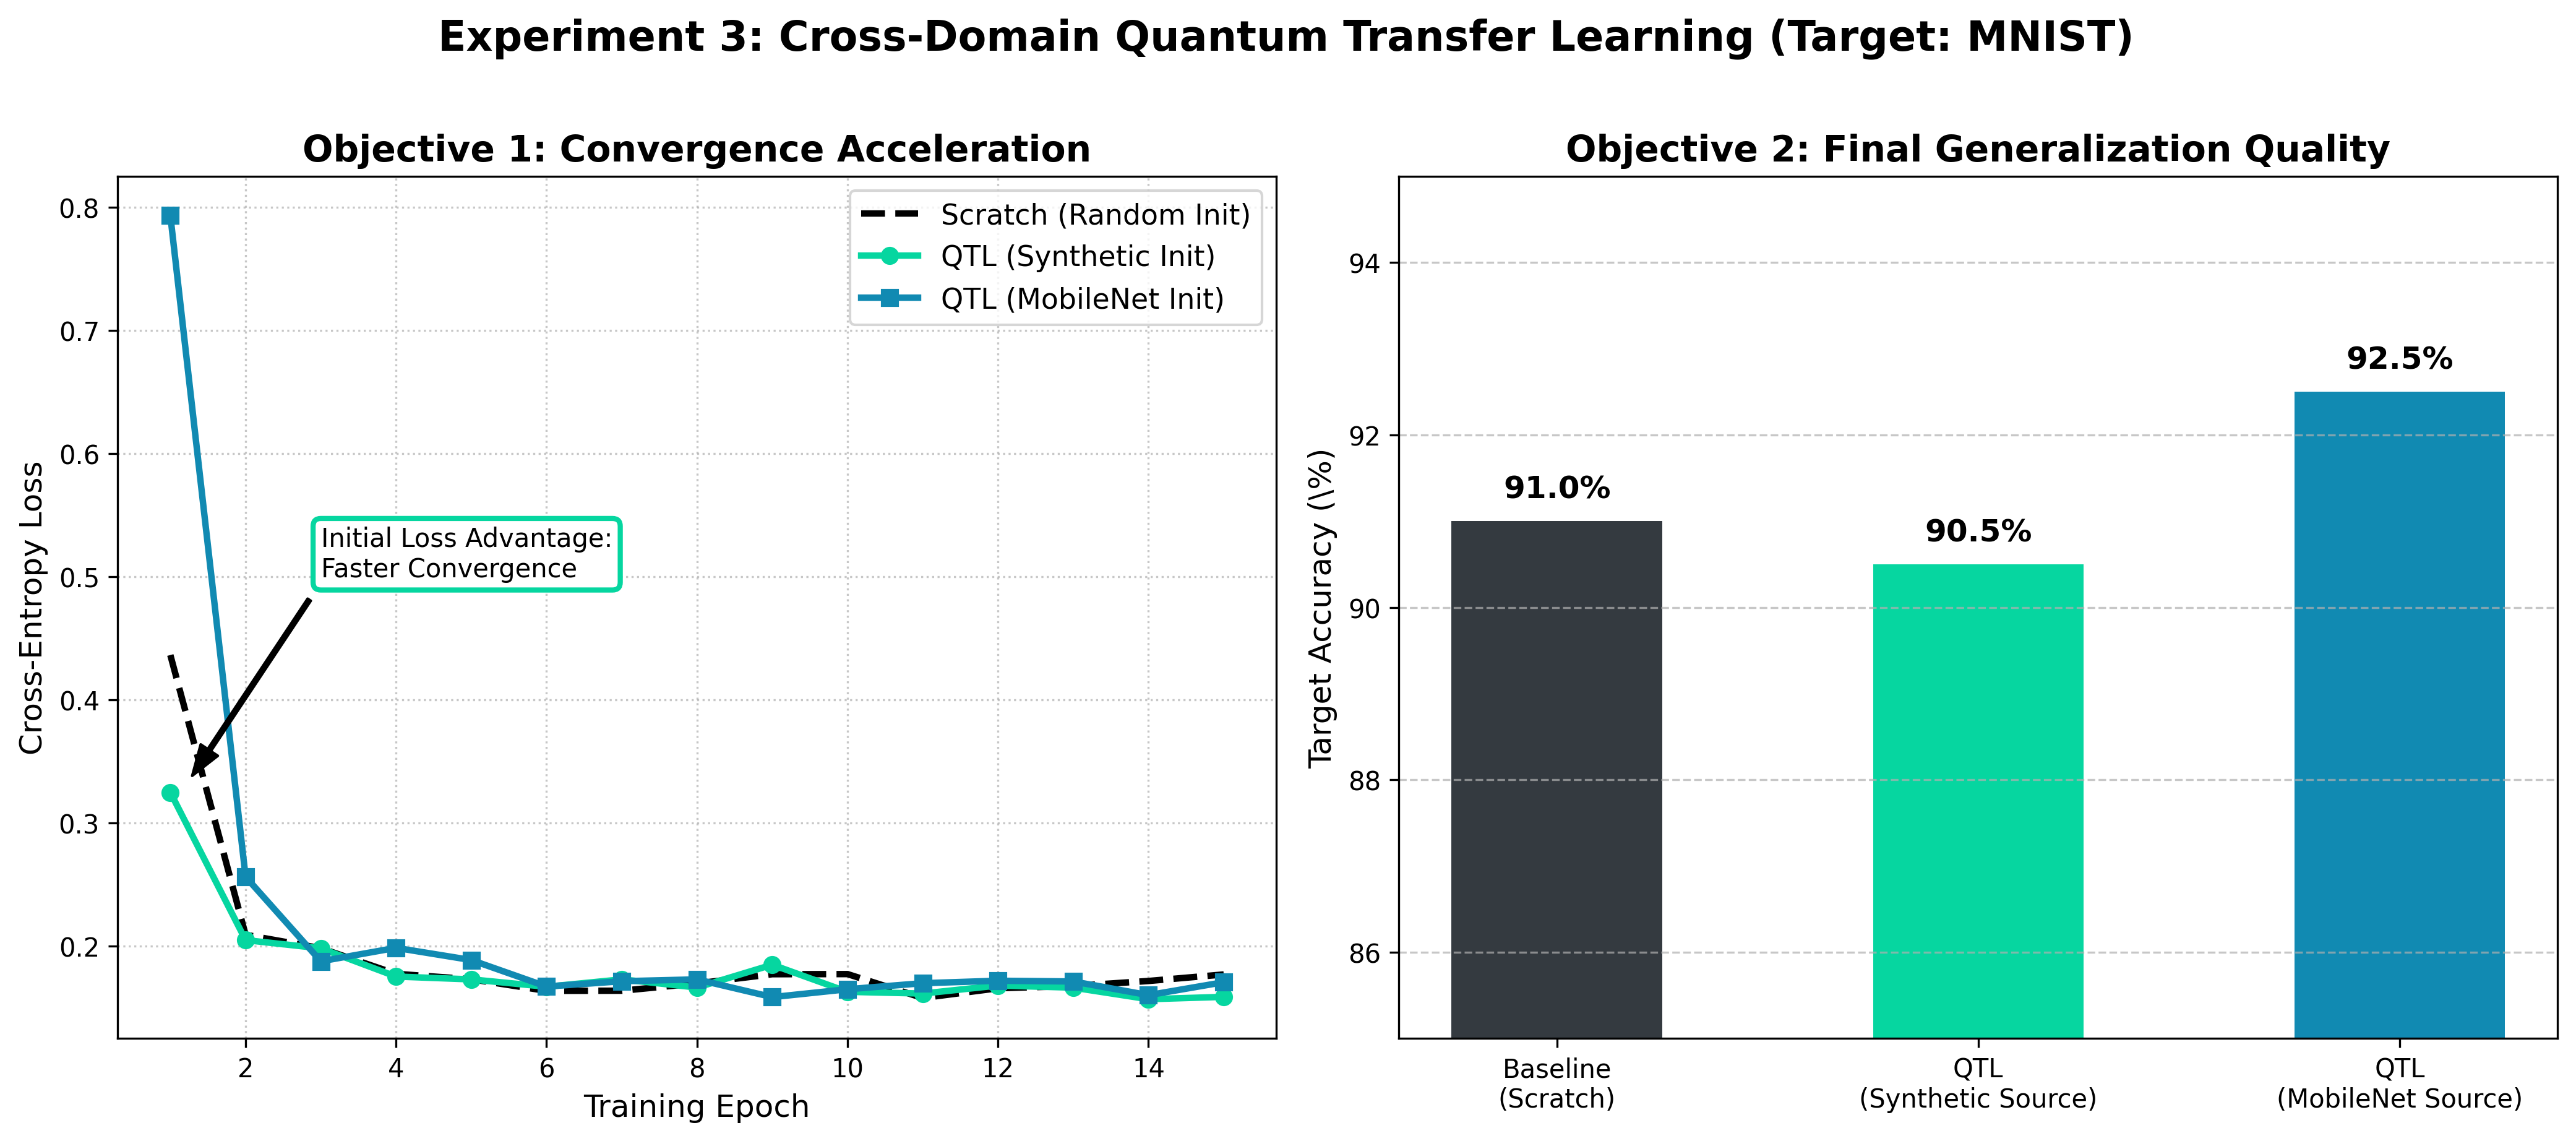
\includegraphics[width=0.90\linewidth]{figure3_convergence.png}
  \caption{Cross-entropy loss during Task~A training (10 epochs) for
    three initialization strategies (TTN ansatz, ideal simulation).
    Synthetic Gaussian pre-training (solid line) reaches lower loss
    values at epoch 5 than random initialization (dashed), indicating
    faster convergence. MobileNet-V2 pre-training (dotted) shows
    intermediate behavior.}
  \label{fig:results_figure3}
\end{figure}

% ============================================================
\section{Conclusions}

This paper evaluated cross-domain pre-training as a strategy to reduce
catastrophic forgetting in sequential variational quantum classifiers.
The main finding is that pre-training a VQC on a synthetic Gaussian
source domain reduces the forgetting drop on Task~A by more than 25\%
relative to random initialization, without requiring replay buffers or
parameter regularization. The effect persists under IBM~Heron~r2 noise,
though the magnitude is reduced.

Among the three circuit architectures tested, the TTN ansatz produces
the lowest forgetting drop in all conditions. Its hierarchical parameter
structure limits the propagation of task-specific gradient updates,
making it the most appropriate choice for QCL scenarios on near-term
hardware.

The noise analysis reveals that IBM~Heron~r2 hardware errors reduce
Task~A accuracy by approximately 5--8 percentage points relative to
ideal simulation, and increase $\Delta_A$ by 3--5 percentage points.
This gap must be closed before QCL methods can transfer from simulation
to physical devices. Hardware-specific mitigation techniques, such as
zero-noise extrapolation or probabilistic error cancellation, are
identified as necessary extensions.

Future work will extend the sequential task length beyond two tasks,
assess the scalability of cross-domain pre-training with increasing
qubit count, and investigate whether structured synthetic sources
(topological graphs, Fourier modes) provide stronger protection than
isotropic Gaussian clusters.

\bibliographystyle{splncs04}
\bibliography{references}

\end{document}
